\section{Motivation and approach\label{section:deductive-motivation}}

Building adequate, complete and consistent process models is not necessarily an easy task. Flawed models can have dreadful consequences in safety-critical areas. The recent usage of process modeling to improve medical safety provides a good example of such area \cite{Clarke:2008, Grando:2009, Damas:2011}; models there should be as error-free as possible. Techniques should therefore be available to support model construction and analysis, in particular for systematically detecting and fixing severe flaws.

A typical analysis technique coming to mind is \emph{model checking} \cite{Clarke:1989}. Model-checking would allow us to verify that a given safety property is satisfied in all process instances. Other kinds of analysis on process models are discussed in \cite{Damas:2011}, including checking the satisfiability of guards; verifying that temporal constraints are met; detecting inaccurate process decisions; and so on. This kind of check should be performed ahead of process enactment.

Verification techniques require a formal semantics for process models. As our guarded hMSCs are an extension of hMSCs, a trace semantics appears natural. This choice also fits the intuition: an event trace can roughly be rephrased in terms of temporal occurrences of tasks. Moreover, a trace semantics for g-hMSCs enables reusing LTS-based tools and techniques \cite{Magee:1999, Giannakopoulou:2003}.

\begin{figure}\centering
\scalebox{0.64}{
  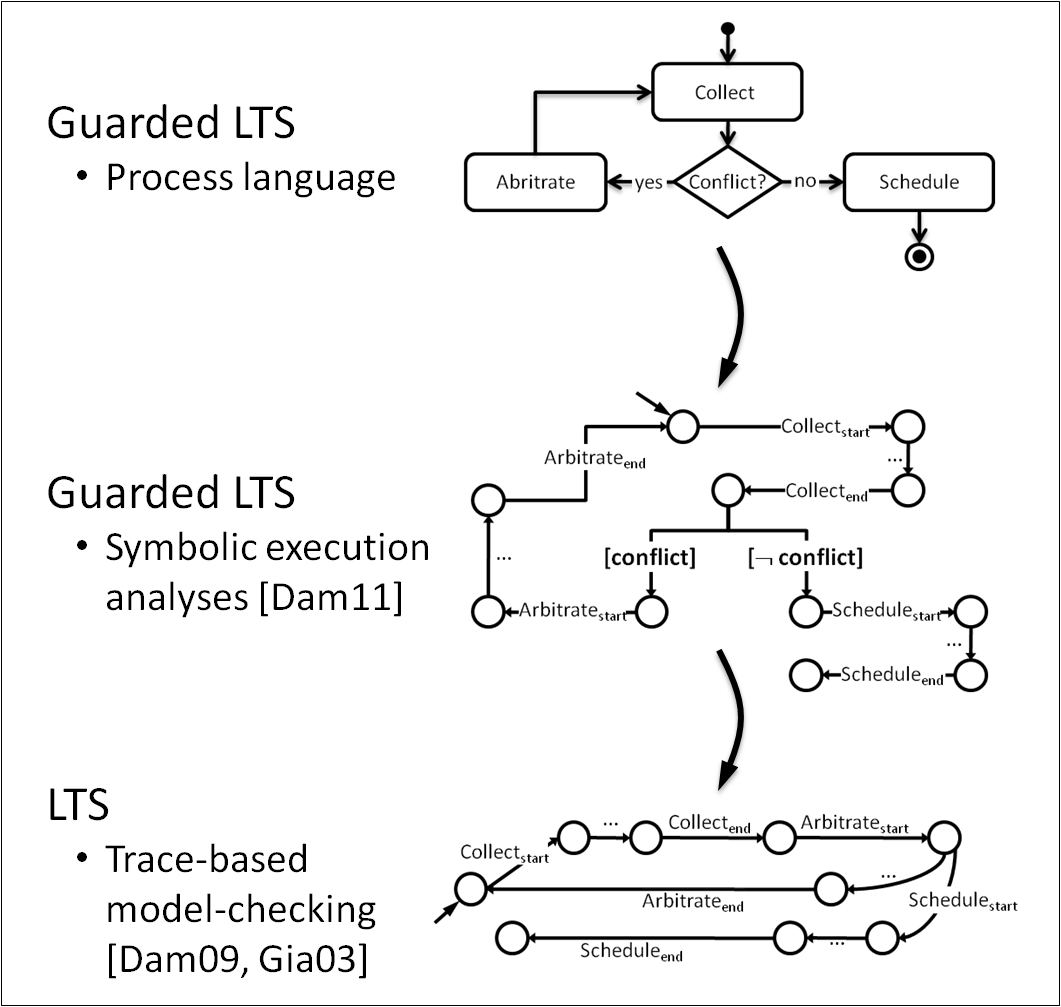
\includegraphics[trim=5mm 2mm 2mm 2mm, clip]{src/3-deductive/images/chapter-overview}
}
\caption{Guarded LTS as an intermediate level between g-hMSC and LTS.\label{image:deductive-chapter-overview}}
\end{figure}

We will only consider the traces of a process globally, that is, as sequences of events seen by an external observer. In other words, in spite of a multi-agent view through message sequence charts, we will not consider agent state machines in isolation. The aim of process modeling is \emph{not} to specify valid executions of the agents themselve, but to capture the control flow of their tasks. 

As a consequence, we will assume a strong sequential composition of g-hMSC nodes and a total ordering of all events inside MSCs (see Section~\ref{subsection:background-hmsc}). In other words, we will assume that agents synchronize with each other when tasks are started and completed. 

To delimit task boundaries in event traces and reason about execution time, each task $T$ will be associated with special events $T_{start}$ and $T_{end}$. These events are assumed to be monitored by all agents; thus, they allow explicitely capturing the required synchronization scheme.

Instead of transforming a guarded hMSC into a LTS directly, we will generate an intermediate form called guarded labeled transition systems (g-LTS). Roughly, a g-LTS is a transition system with guards or events on transitions. It is a structured form of LTS aimed to avoid state explosion. This intermediate form is therefore easier to understand and supports different types of analysis at an abstract level; it may also facilitate code generation for process enactment. 

Figure~\ref{image:deductive-chapter-overview} illustrates the three abstraction levels provided by g-hMSC, g-LTS and LTS, respectively. Analyses about guards, temporal constraints and the like are performed at the g-LTS level. They rely on a generalization of the symbolic execution algorithm used to decorate a LTS with assertions on fluents (see Section \ref{section:background-fluents}). For details about such analyses at the g-LTS level, see \cite{Damas:2011}. Trace-based model-checking can be performed at the LTS level, using slight adaptations of existing tools such as LTSA \cite{Magee:1999} (see Section \ref{section:tool-model-checker}).

Our two derivation algorithms for transforming a guarded hMSC to a guarded LTS then to a LTS are detailed in Section \ref{section:deductive-glts-to-lts}. Section \ref{section:deductive-glts} first introduces guarded LTS formally; it also provides a few operators for manipulating them.
